\documentclass{article}

\usepackage{geometry}
\usepackage{amsmath}
\usepackage{graphicx, eso-pic}
\usepackage{listings}
\usepackage{hyperref}
\usepackage{multicol}
\usepackage{fancyhdr}
\pagestyle{fancy}
\fancyhf{}
\hypersetup{ colorlinks=true, linkcolor=black, filecolor=magenta, urlcolor=cyan}
\geometry{ a4paper, total={170mm,257mm}, top=40mm, right=20mm, bottom=20mm, left=20mm}
\setlength{\parindent}{0pt}
\setlength{\parskip}{0.3em}
\renewcommand{\headrulewidth}{0pt}
\rfoot{\thepage}
\lfoot{Seleksi IEEEXtreme 15.0 ITB}
\lstset{
    basicstyle=\ttfamily\small,
    columns=fixed,
    extendedchars=true,
    breaklines=true,
    tabsize=2,
    prebreak=\raisebox{0ex}[0ex][0ex]{\ensuremath{\hookleftarrow}},
    frame=none,
    showtabs=false,
    showspaces=false,
    showstringspaces=false,
    prebreak={},
    keywordstyle=\color[rgb]{0.627,0.126,0.941},
    commentstyle=\color[rgb]{0.133,0.545,0.133},
    stringstyle=\color[rgb]{01,0,0},
    captionpos=t,
    escapeinside={(\%}{\%)}
}

\begin{document}

\begin{center}
    \section*{Pohon dan Faktor} % ganti judul soal

    \begin{tabular}{ | c c | }
        \hline
        Batas Waktu  & 1 s \\    % jangan lupa ganti time limit
        Batas Memori & 256 MB \\  % jangan lupa ganti memory limit
        \hline
    \end{tabular}
\end{center}

\subsection*{Deskripsi}
Diberikan \href{https://en.wikipedia.org/wiki/Tree_(graph_theory)#Rooted_tree}{\textit{rooted tree}} dengan $N$ \textit{node} bernomor $1$ sampai $N$. \textit{Root tree} ini adalah \textit{node} bernomor $1$. 

Jawablah $Q$ pertanyaan, pertanyaan ke-$i$ berbunyi "Berapa banyak \textit{node} di \textit{subtree node} $X_i$ yang nomornya dibagi habis $Y_i$?".

Sebuah \textit{node} $U$ berada di \textit{subtree node} $V$ apabila satu-satunya \textit{simple path} dari $U$ ke \textit{root} melewati $V$.

\subsection*{Format Masukan}
Baris pertama masukan berisi sebuah bilangan bulat $N$ $(1 \leq N \leq 5 \times 10^4)$ - banyak \textit{node} di \textit{tree}.

Masukan dilanjutkan dengan $N-1$ baris. Baris ke-$i$ berisi dua bilangan bulat $U_i$ dan $V_i$ $(1 \leq U_i, V_i \leq N)$ dan menyatakan bahwa terdapat \textit{edge} yang menghubungkan \textit{node} $U_i$ dan \textit{node} $V_i$. Kumpulan \textit{node} dan \textit{edge} dijamin membentuk sebuah \textit{tree}.

Baris berikutnya berisi satu bilangan bulat $Q$ $(1 \leq Q \leq 5 \times 10^4)$ - banyak pertanyaan.

Masukan dilanjutkan dengan $Q$ baris. Baris ke-$i$ berisi dua bilangan bulat $X_i$ dan $Y_i$ $(1 \leq U_i, V_i \leq N)$ - nilai pada pertanyaan ke-$i$.

\subsection*{Format Keluaran}
Keluaran terdiri atas $Q$ baris. Baris ke-$i$ berisi bilangan bulat yang menyatakan jawaban pertanyaan ke-$i$.

\begin{multicols}{2}
\subsection*{Contoh Masukan}
\begin{lstlisting}
7
1 2
3 2
6 1
2 5
6 7
7 4
7
2 1
1 2
1 3
6 4
5 5
3 6
4 7
\end{lstlisting}
\null
\columnbreak
\subsection*{Contoh Keluaran}
\begin{lstlisting}
3
3
2
1
1
0
0
\end{lstlisting}
\vfill
\null
\end{multicols}

\newpage
\subsection*{Penjelasan}
Pohon pada contoh berbentuk seperti berikut.
\begin{center}
    \fbox{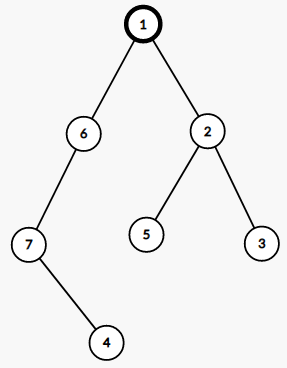
\includegraphics[scale=0.7]{graph.png}}
\end{center}
\textit{Node} $5$, $2$, dan $3$ berada di \textit{subtree node} $2$. Selain itu, nomor \textit{node} $5$, $2$, dan $3$ habis dibagi $1$. Oleh sebab itu, jawaban pertanyaan ke-$1$ adalah $3$.

\end{document}